\documentclass[12pt]{article}

\usepackage[fleqn]{amsmath}
\usepackage{amssymb}
\usepackage{amsthm}
\usepackage{graphicx}
\usepackage{float}
\theoremstyle{plain}     %------- 'regular' theorem types
\newtheorem{thm}{Theorem}[section]
\newtheorem{cor}[thm]{Corollary}
\newtheorem{lemma}[thm]{Lemma}
\newtheorem{prop}[thm]{Proposition}
\newtheorem{example}[thm]{Example}
\newtheorem{exer}[thm]{Exercise}
\newtheorem{define}[thm]{Definition}
\usepackage[top=2cm, left=2cm, right=2cm]{geometry} 
\usepackage{parskip}
\setlength{\parindent}{0in}
\usepackage{floatflt}
\usepackage{multicol}
\usepackage{tabu}
\usepackage[hidelinks]{hyperref}
\hypersetup{
	urlcolor=blue}

%%%%%%%%%%%%%%%%%%%%%%
%%%%%%%%%%%%%%%%%%%%%%%
%%%%%%%%%%%%%%%%%%%%%%%%
\begin{document}
\large
%subject
City Semester  \hspace{8cm} Name:\makebox[6cm]{\hrulefill}
\\
%specific topic
Measuring Income Inequality\\
\normalsize 
\emph{Complete all work on a separate sheet of paper with exercises clearly labeled and all reasoning and work given.}\\[.5cm]
%\emph{Show all work for full credit.}
\begin{enumerate}
	\item The Lorenz curve is the name given to a curve that attempts to represent the distribution of wealth or income in a community. Each point $(x,y)$ on the Lorenz curve represents the percentage of the total income $y$ held by the bottom $x$ percent of households  when ranked by income. For example the point if $(0.2,0.1)$ is on the Lorenz curve for a community, it would mean that for this community the bottom 20\% of households ranked by income earn 10\% of the total income earned by the community.
		\begin{enumerate}
		\item What is the domain of the Lorenz curve?
		\item What is the range of the Lorenz curve?
		\item If everyone in the community earned the same income, what would the Lorenz curve look like?
		\item If everyone int the community except Alice earns 0 income, what would the Lorenz curve look like? (note:the curve does not have to be continuous.)
		
		\end{enumerate}
		\item The Gini coefficient is a frequently used  as a coarse measure of the inequality of wealth distribution among a community. There are many variants and the wikipedia entry is a very readable and good introduction to all the varied forms and applications of the idea. Let us recall the Lorenz curve that arises in 1c and call this the line of equality. The gini coefficient is calculated by finding the area between a community's Lorenz curve and the line of equality and dividing that by 0.5.
			\begin{enumerate}
				\item In the figure below if $A$ has area 0.2 calculate the gini coefficient.
					\begin{figure}[H]
						\hspace{2cm}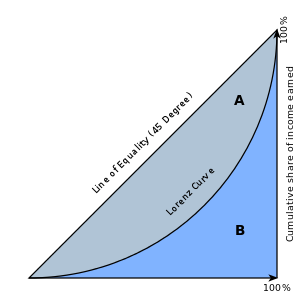
\includegraphics[scale=.4]{1.png}
					\end{figure}
					\item In the community of 1c what would the gini coefficient be?
					\item In the community of 1d what would the gini coefficient be?
					\item What does a gini coefficient close to 1 mean? What does it mean if it is close to 0?
			\end{enumerate}
		\item Let's calculate the gini coefficient for new york city.
			\begin{enumerate}
			\item The fathom file has adjusted gross income by household for nyc 2013 divided by deciles. Plot the data to generate the lorenz curve for nyc.
			\item So we are going to fit this data to an exponential model. Find the exponential model that best fits the data.
			\item Now we need to be able to find the area between the lorenz curve you found and the line of equality. To do this ask wolfram alpha to find the area between the curves.
			\item Now we can calculate the gini coefficient. How do you think nyc compares to the nation at large? What about to other countries. Look up some gini coefficients for other countries. Note down one that has `more' inequality and one that has `less'.
			\end{enumerate}
\end{enumerate}
	
\end{document} 